
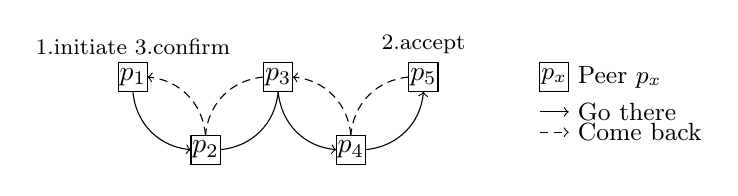
\begin{tikzpicture}[scale=1.05]

  \footnotesize
  \draw (0pt,5pt)node[anchor=south]{1.initiate 3.confirm};
  \draw (100pt,5pt)node[anchor=south]{2.accept};

  \normalsize
  \draw[fill=white] (0pt, 0pt) node{$p_1$} +(-5pt,-5pt) rectangle +(5pt,5pt);
  \draw[fill=white] (25pt,-25pt) node{$p_2$} +(-5pt,-5pt) rectangle +(5pt,5pt);
  \draw[fill=white] (50pt, 0pt) node{$p_3$} +(-5pt,-5pt) rectangle +(5pt,5pt);
  \draw[fill=white] (75pt,-25pt) node{$p_4$} +(-5pt,-5pt) rectangle +(5pt,5pt);
  \draw[fill=white] (100pt, 0pt) node{$p_5$} +(-5pt,-5pt) rectangle +(5pt,5pt);


  \draw[->] ( 0pt,-5pt) to[out=-85,in=175] (20pt,-25pt);
  \draw[->, densely dashed] (25pt, -20pt) to[out=95,in=-5] ( 5pt, 0pt);
  \draw     ( 30pt, -25pt) to[out=5,in=-95] (50pt,-5pt);
  \draw[densely dashed] ( 45pt, 0pt) to[out=185,in=85] (25pt, -20pt);
  \draw[->] (50pt, -5pt) to[out=-85,in=175] (70pt,-25pt);
  \draw[->, densely dashed] (75pt, -20pt) to[out=95,in=-5] (55pt,0pt);
  \draw[->] (80pt, -25pt) to[out=5pt,in=-95] (100pt,-5pt);
  \draw[densely dashed] (95pt, 0pt) to[out=185,in=85] (75pt, -20pt);
%%  \draw[->, densely dashed] (-70pt, 0pt) -- (-30pt, 0pt); %% u1 -> u4
%%  \draw[->, densely dashed] (-5pt, 30pt) -- (-70pt, 5pt); %% u3 -> u1
%%  \draw[->, densely dashed] (30pt, -5pt) to[out=-85,in=-95](-70pt,-5pt);%%u5 u1

  \small 
  \begin{scope}[shift={(140pt,0pt)}]
    \draw[fill=white](5pt, 0pt)node{$p_x$}+(-5pt,-5pt) rectangle +(5pt,5pt);
    \draw (10pt,0pt) node[anchor=west]{Peer $p_x$};
    \draw[->](0pt, -12pt)--(10pt, -12pt) node[anchor=west]{Go there};
    \draw[->, densely dashed](0pt, -19pt)--(10pt, -19pt)
    node[anchor=west]{Come back};    
  \end{scope}
  
\end{tikzpicture}